\documentclass[11pt, a4paper, oneside]{ctexart}
\usepackage{indentfirst, amsmath, amsthm, amssymb, graphicx, float, subfigure, geometry, setspace, xfrac, tikz-cd, enumerate}
\usepackage[bookmarks=true, colorlinks, citecolor=blue, linkcolor=black]{hyperref}
\ctexset{
    section = {
        format = {\Large\bfseries},
    }
}

% 导言区

\title{Note 02}
\author{zero-point\_}
\setlength{\parindent}{4ex}
\pagestyle{plain}
\geometry{left=2.54cm, right=2.54cm, top=3.18cm, bottom=3.18cm}
\setstretch{1.5}

\newtheorem{theorem}{定理}[section]
\newtheorem{corollary}[theorem]{推论}
\newtheorem{definition}[theorem]{定义}
\newtheorem{example}[theorem]{例}
\newtheorem{lemma}[theorem]{引理}
\newtheorem{proposition}[theorem]{命题}
\newtheorem{remark}[theorem]{注}

\newcommand{\C}{\mathbb{C}}
\newcommand{\N}{\mathbb{N}}
\newcommand{\Q}{\mathbb{Q}}
\newcommand{\R}{\mathbb{R}}
\newcommand{\T}{\mathbb{T}}
\newcommand{\Z}{\mathbb{Z}}
\newcommand{\cA}{\mathcal{A}}
\newcommand{\cO}{\mathcal{O}}
\newcommand{\Id}{\mathrm{Id}}
\newcommand{\tr}{\mathrm{tr}}
\newcommand{\abs}[1]{\left|{#1}\right|}
\renewcommand{\v}[1]{\mathbf{#1}}

\begin{document}
	\maketitle
    \section{内容安排}
    \begin{itemize}
        \item 符号序列空间
        \item 移位映射与拓扑 Markov 链
        \item 编码与 Markov 分割
    \end{itemize}

    \section{符号序列空间}
    上次在研究扩张映射时，我们将它转化为了 $k$-进制小数的空间. 本讲我们将形式化这一概念.
    \begin{definition}[符号序列]
        设正整数 $N\geq 2$，考虑字码（为方便起见，设字码为 $\{0,1,\ldots,N-1\}$），则定义双向符号序列 $\Omega_N=\{\omega=(\ldots,\omega_{-1},\omega_0,\omega_1,\ldots)\mid \omega_i\in\{0,1,\ldots,N-1\},\; i\in\Z\}={\{0,1,\ldots,N-1\}}^{\Z}$. 类似的可以定义单向符号序列 $\Omega_N^R={\{0,1,\ldots,N-1\}}^{\N_0}$（从 $0$ 开始，没有负下标）. 我们为 $\{0,1,\ldots,N-1\}$ 赋予离散拓扑，为 $\Omega_N,\Omega_N^R$ 赋予由此产生的乘积拓扑.
    \end{definition}
    \begin{remark}
        若视 $\{0,1,\ldots,N-1\}=\Z/N\Z$，则符号序列自然产生一个紧 Abelian 拓扑群（承认 Tychonoff 定理时）.
    \end{remark}
    \begin{definition}[圆柱]
        设 $n_1<n_2<\cdots<n_k$ 以及字码 $\alpha_1,\ldots,\alpha_k\in\{0,1,\ldots,N-1\}$，定义圆柱 $C_{\alpha_1,\ldots,\alpha_k}^{n_1,\ldots,n_k}=\{\omega\in\Omega_N\mid \omega_{n_i}=\alpha_i,i\in\{1,\ldots,k\}\}$，$k$ 是圆柱的秩.
    \end{definition}
    \begin{remark}
        \begin{itemize}
            \item 根据乘积拓扑的定义，圆柱构成了拓扑基.
            \item 圆柱也是闭的（为什么？）.
            \item 圆柱的交若非空则也是圆柱.
        \end{itemize}
    \end{remark}
    \begin{definition}[符号序列空间的度量]
        任取 $\lambda>1$，则 $d_{\lambda}(\omega,\omega')=\sum\limits_{n=-\infty}^{\infty}\frac{\abs{\omega_n-\omega_n'}}{\lambda^{\abs{n}}}$ 定义了一个度量（请验证）. 对于足够大的 $\lambda$（例如 $\lambda=2N$），任意的对称圆柱 $C_{\alpha_{-n},\ldots,\alpha_n}^{-n,\ldots,n}$ 都是球.
    \end{definition}
    \begin{remark}
        \begin{itemize}
            \item 这个度量与乘积拓扑相合.
            \item $\Omega_N$ 是完美的（每个点都是空间中的聚点）、完全不连通（连通集必然是单点）的紧空间. 因此它和 $[0,1]$ 区间中对应构造的 Cantor 集是同胚的.
            \item $\Omega_N$ 实际上可以定义出一个 Hölder 结构（本讨论班貌似用不上它，感兴趣的可以看书）.
        \end{itemize}
    \end{remark}

    \section{移位映射与符号动力系统}
    \begin{definition}[左移映射]
        设左移映射 $\sigma_N:\Omega_N\to \Omega_N;\; \omega\mapsto \omega'$，使得 $\omega'_n=\omega_{n+1}$. 在双向符号序列空间中这显然是同胚（请验证连续性条件），而单向符号序列空间中，类似构造得到的映射 $\sigma_N^R$ 是不可逆连续满射.
    \end{definition}

    \begin{proposition}[周期点分析]
        $\sigma_N$ 的周期点在 $\Omega_N$ 上稠密，且 $P_n(\sigma_N)=N^n$，且 $\sigma_N$ 拓扑混合.
    \end{proposition}
    \begin{proof}[证明提示]
        对于第一个命题，只需在每个圆柱内构造一个周期点即可；第二个命题显然；对于第三个命题，由于每个圆柱内都包含了一个对称圆柱，于是我们只需任取两个对称圆柱并证明拓扑混合性，对足够大的每个 $N$，构造是容易的.
    \end{proof}
    \begin{remark}
        上述命题对 $\sigma_N^R$ 同样有效（请证明）.
    \end{remark}

    \begin{definition}[符号动力系统]
        设 $K\subset \Omega_N$ 是 $\sigma_N$ 的不变闭集，则 $\sigma_N|_{K}$ 称为符号动力系统（对单向符号序列空间同理，也称符号动力系统）.
    \end{definition}

    \section{拓扑 Markov 链}
    接下来我们介绍最简单的非平凡符号动力系统.
    \begin{definition}
        给定 $0-1$ 矩阵 $A\in M_N(\{0,1\})$，设 $\Omega_A=\{\omega\in\Omega_N\mid a_{\omega_n\omega_{n+1}}=1,\; \forall\; n\in\Z\}$（不变性显然；请用列闭定义验证闭性），则 $\sigma_A=\sigma_N|_{\Omega_A}$ 称为拓扑 Markov 链，也叫有限型子移位.
    \end{definition}
    \begin{remark}
        就像高中学的 Markov 链一样，我们也可以用图 $G_A$ 来表示，这时对应矩阵 $A$ 称为邻接矩阵. 我们会把 $G_A$ 中的有限/无限长度通路（也可以用对应的符号列表示）称为容许路径/序列.
    \end{remark}

    \begin{lemma}
        任意给定 $i,j\in\{0,1,\ldots,N-1\}$，则长度为 $m+1$ 的、起点为 $i$、终点为 $j$ 的容许路径数量 $N_{ij}^{m}=a_{ij}^{m}$，这里 $a_{ij}^{m}$ 是 $A^m$ 的 $i$ 行 $j$ 列值.
    \end{lemma}
    \begin{proof}[证明提示]
        这是简单的离散数学习题，使用归纳法即证.
    \end{proof}

    \begin{corollary}[$\sigma_A$ 的周期点]\label{Cor4.4}
        $P_n(\sigma_A)=\tr(A^n)$
    \end{corollary}

    \begin{definition}[传递矩阵]
        $0-1$ 矩阵 $A$ 称为传递矩阵，若存在 $m>0$ 使得 $A^m$ 的每个元素都是正数. $\sigma_A$ 称为传递的，若 $A$ 是传递的.
    \end{definition}
    \begin{remark}
        注意传递性与拓扑传递性只是撞名了，定义上并不相同，虽然命题~\ref{Prop4.9} 说明了传递的映射一定是拓扑传递的.
    \end{remark}

    \begin{lemma}\label{Lemma4.7}
        若 $A^m$ 的每个元素都是正数，则 $\forall\; n\geq m$，$A^n$ 的每个元素都是正数.
    \end{lemma}
    \begin{proof}
        只需证 $n=m+1$ 情形. 首先反证法可以证明，若 $A^m$ 的每个元素都是正数，则 $\forall\; j\in\{0,\ldots,N-1\},\; \exists\; k\in \{0,\ldots,N-1\},\; a_{kj}=1$. 接下来代入矩阵乘法的公式即证.
    \end{proof}

    \begin{lemma}[传递性与周期点]\label{Lemma4.8}
        设 $\sigma_A$ 传递，$\alpha=(\alpha_{-k},\ldots,\alpha_k)$ 是容许路径，则 $\Omega_A\cap C_{\alpha}^{k}=:C_{\alpha,A}^{k}$ 不仅非空，还包含一个周期点. 于是，$\sigma_A$ 的周期轨道在 $\Omega_A$ 中稠密.
    \end{lemma}
    \begin{proof}
        $\alpha$ 给出从 $\alpha_{-k}$ 到 $\alpha_k$ 的通路，而由传递性，$\alpha_k$ 到 $\alpha_{-k}$ 之间存在长度为 $m$ 的通路，于是可以构造周期点.
    \end{proof}

    \begin{proposition}[传递性与拓扑混合性]\label{Prop4.9}
        设 $\sigma_A$ 传递，则它是拓扑混合的.
    \end{proposition}
    \begin{proof}
        证明与引理~\ref{Lemma4.8} 类似，但要注意使用引理~\ref{Lemma4.7} 的结论，才可以构造任意足够长的通路.
    \end{proof}

    \begin{definition}[$n$-步拓扑 Markov 链]
        设 $0-1$ 张量 $\cA:{\{1,\ldots,N\}}^{n+1}\to \{0,1\}$，定义闭不变集 $\Omega_{\cA}=\{\omega\in\Omega_N\mid \cA(\omega_m,\ldots,\omega_{m+n})=1,\;\forall\; m\in\Z\}$，则 $\sigma_{\cA}=\sigma_N|_{\Omega_{\cA}}$ 称为 $n$-步拓扑 Markov 链.
    \end{definition}
    \begin{remark}
        通过考虑新的字码 ${\{1,\ldots,N\}}^n$，可以将 $n$-步拓扑 Markov 链转为普通的拓扑 Markov 链（对应的邻接矩阵需要考虑哪两个因素？）.
    \end{remark}

    接下来，设 $\lambda_1,\ldots,\lambda_N$ 是 $A$ 的特征值，按照模长单调不增排序. 于是推论~\ref{Cor4.4} 给出 $P_n(\sigma_A)=\sum\limits_{i=1}^{N}\lambda_i^n$. 对于传递矩阵，我们可以给出更精确的特征值估计.

    \begin{theorem}[Perron-Frobenius]\label{Thm4.12}
        设非负矩阵 $L\in M_N(\R_{\geq 0})$，且满足 $\exists\; n>0,\; L^n$ 的每个元素都是正数，则 $L$ 的所有单位特征向量中，有且仅有一个（设为 $\v{e}$）坐标全为正数，而且其他各个的坐标都至少有一个负数. 而且，$\v{e}$ 对应的特征值 $\lambda$ 是正的单特征根，而且模长比所有其他的特征值模长更大.
    \end{theorem}
    \begin{remark}
        本定理涉及比较复杂的凸集的分析，而且与主线关系不大，因此我们直接承认它，并给出它的以下重要推论.
    \end{remark}
    \begin{corollary}
        传递 $0-1$ 矩阵 $A$ 满足：$P_n(\sigma_A)=\lambda_0^n+\mu_n$，这里 $\lambda_0$ 是最长模长的特征根，且 $\lambda_0>1$，而我们还有估计 $\abs{\mu_n}=O(\lambda^n)$，这里 $\lambda<\lambda_0$ 是一个正数.
    \end{corollary}
    \begin{proof}
        唯一不平凡的是 $\lambda_0>1$. 设 $x$ 是 $\lambda_0$ 的特征向量，则 $A^n x=\lambda_0^n x$，也即 $\lambda_0^n x_i=\sum\limits_{j=0}^{N-1}a_{ij}^n x_j$，由于传递性知 $n$ 足够大时 $a_{ij}^n\geq 1$，于是 $\lambda_0^n x_i\geq x_i$，于是 $\lambda_0>1$.
    \end{proof}

    \section{Markov 分割}
    符号动力系统架构简单，性质清晰，那它和其他的动力系统如何起到联系？这里我们介绍 Markov 分割方法，它将其他的动力系统的问题通过半共轭转化为符号动力系统的问题，这是动力系统中极其常见的方法.

    \begin{example}[双曲环面自同构]
        我们仍然研究 $F=\begin{bmatrix}
            2&1\\
            1&1\\
        \end{bmatrix}$ 对应的环面自同构. 我们先将环面变形为下图的样子，得到两个矩形 $R^{(1)},R^{(2)}$ 叠起来（借用教材的图）：
        \begin{figure}[H]
            \centering
            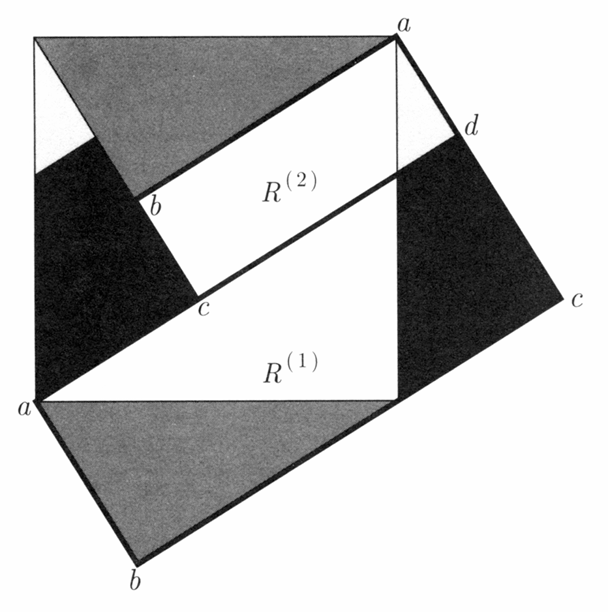
\includegraphics[width=0.5\textwidth]{0201.png}
        \end{figure}

        接下来考虑像 $F(R^{(1)}),F(R^{(2)})$ 与原矩形的相交情况，我们仍然在 $\R^2$ 上工作，但请时刻记得要投影到 $\T^2$ 上得到结论.
        \begin{figure}[H]
            \centering
            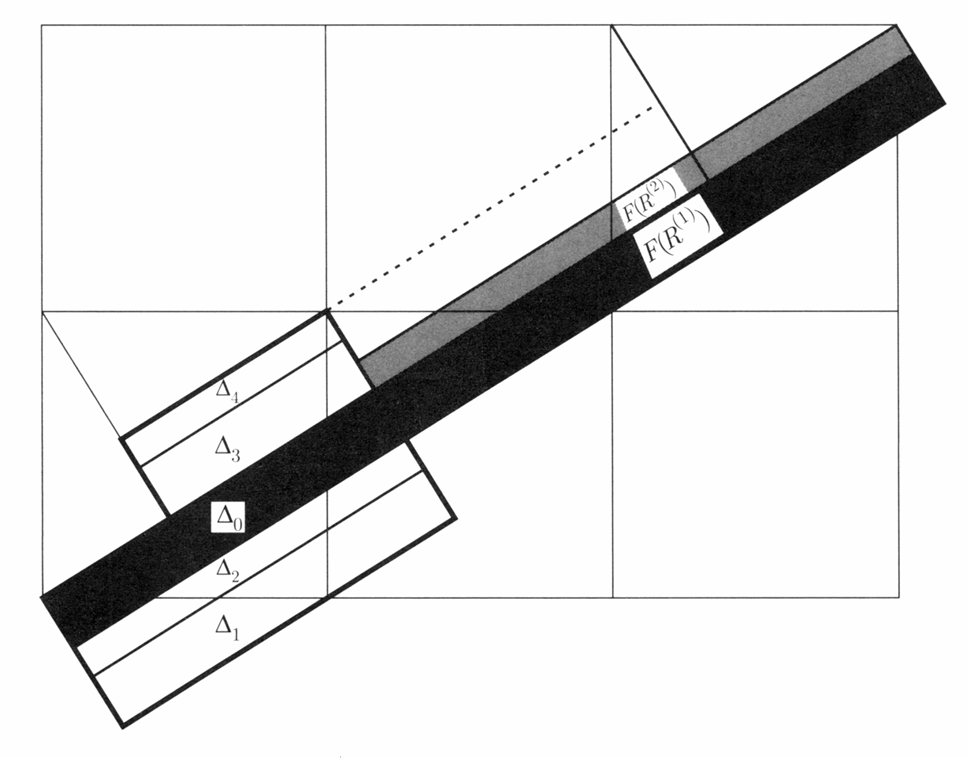
\includegraphics[width=0.5\textwidth]{0202.png}
        \end{figure}

        我们于是划分出 $\Delta_0,\ldots,\Delta_4$，其中 $\Delta_0,\Delta_1,\Delta_3\subset F(R^{(1)})$，另外两个包含于 $F(R^{(2)})$（请通过计算验证 $F(R^{(1)}),F(R^{(2)})$ 的像的确如图中画的那样）. 接下来，我们设 $\Delta_{i_{-1} i_0}=F(\Delta_{i_{-1}})\cap \Delta_{i_0}$，以此类推，设 $\Delta_{i_{-k}\cdots i_0}=F(\Delta_{j_{-k+1}\cdots j_{0}})\cap \Delta_{i_0}$，其中 $j_l=i_{l-1}$（注意这里下标顺序指的是绝对位置，而不是相对关系）；又设 $\Delta_{\cdots i_0 i_1}=\Delta_{\cdots i_0}\cap F^{-1}(\Delta_{i_1})$，以此类推，设 $\Delta_{\cdots i_0\cdots i_k}=\Delta_{\cdots i_0}\cap F^{-1}(\Delta_{j_0\cdots j_{k-1}})$，其中 $j_l=i_{l+1}$. 于是每个 $\Omega_5$ 中的元素 $\omega$ 都至多对应一个矩形套（有可能无法对应，为什么？） $\Delta_{\omega}$，且 $F(\Delta_{\omega})=\Delta_{\sigma_5(\omega)}$. 通过压缩性与几何级数的计算（在特征方向赋予坐标后就可以计算），我们知道每个 $\Delta_{\omega}$ 都可以唯一确定一个点 $p$；设 $A=\begin{bmatrix}
            1&1&0&1&0\\
            1&1&0&1&0\\
            1&1&0&1&0\\
            0&0&1&0&1\\
            0&0&1&0&1\\
        \end{bmatrix}$（对应的，考虑 $F(\Delta_i)$ 与哪几个 $\Delta_j$ 相交），于是可以发现只要 $\omega\in \Omega_A$ 就有 $\Delta_{\omega}$ 对应了一个矩形套，从而唯一对应了点 $p$. 设 $h:\Omega_A\to \T^2$ 满足 $h(\omega)=p$，这是满射但不是单射（考虑边界；教材有更精确的刻画），于是 $F\circ h=h\circ \sigma_A$.

        通过计算特征值，我们发现 $P_n(\sigma_A)=P_n(F)+2$，也就是说多出了两个周期点. 容易发现，$A$ 的不动点是全 $0$ 列、全 $1$ 列和全 $4$ 列，而它们在 $h$ 下的像都是 $0$ 点，于是我们推出：$h$ 将非不动点的周期点双射地映到 $\T^2$ 中.
    \end{example}

    \begin{remark}
        事实上，在第 01 讲中，我们已经使用了 Markov 分割来解决均匀扩张映射的问题. 请理解为什么三进制小数是一种 Markov 分割.
    \end{remark}

    \begin{remark}
        采用连分数形式，我们也可以为小数建立符号动力系统的对应. 有关连分数的内容相当复杂，例如，其中一部分内容可以用热力学形式描述.
    \end{remark}

    \begin{theorem}[扩张映射的拓扑共轭]
        所有度数（拓扑度数）为 $k$ 的圆上的扩张映射 $f$（也即 $\exists\; \mu>1$ 使得 $\abs{f'}\geq\mu$；由紧性知等价于 $\abs{f'}>1$）都与 $E_k$ 拓扑共轭.
    \end{theorem}
    \begin{proof}
        不妨设 $k>1$. 首先我们容易证明：$f$ 存在 $\R\to \R$ 的提升 $F$，且 $F$ 的不动点 $p\in [-\frac{1}{2},\frac{1}{2}]$. 接下来记 $\Delta_n^m=[\frac{m}{k^n},\frac{m+1}{k^n}],\; n\in\Z_{\geq 0},0\leq m\leq k^n-1$，于是 $E_k\Delta_n^m=\Delta_{n-1}^{m'}$，其中 $m'=m\% k^{n-1}$. 记 $\xi_n=\{\Delta_n^0,\ldots,\Delta_n^{k^n-1}\}$ 是 $S^1$ 的分割；我们的目的是构造 $f$ 的分割 $\eta_n=\{\Gamma_n^0,\ldots,\Gamma_n^{k^n-1}\}$，并通过两列分割的对应最后给出点的对应.

        首先构造 $\eta_1$，这里只需取 $\Gamma_1^{t}=\pi(F^{-1}([p+t,p+t+1]))$，其中 $\pi$ 是 $\R\to \R/\Z$ 的商映射. 设 $a_1^t=F^{-1}(p+t)$，于是归纳定义 $a_n^{km+i}$（$0\leq m\leq k^{n-1}-1$ 且 $0\leq i<k$） 满足 $a_{n-1}^m\leq a_n^{km+i}<a_{n-1}^{m+1}$ 且 $\pi(F(a_n^{km+i}))=\pi(a_{n-1}^{m'})$，定义 $\Gamma_n^m=\pi([a_n^m,a_n^{m+1}])$，于是 $f(\Gamma_n^m)=\Gamma_{n-1}^{m\% k^{n-1}}$，而 $f(\Gamma_1^m)=S^1=\Gamma_0^0$. 由于 $f$ 的严格单调性，$f^n$ 在 $\Gamma_n^m$ 内部是单射，于是由于 $f$ 的扩张性知 $\abs{\Gamma_n^m}\leq \mu^{-n}$，于是 $\{a_n^m\}$ 点列稠密（扩张条件的唯一作用就是直接保证了点列的稠密性）.

        最后，设 $h(a_n^m)=\frac{m}{k^n}$，这一对应是单调的，且由于点列 $\{a_n^m\}$ 的稠密性，这一对应可以唯一连续延拓为 $h:[p,p+1]\to [0,1]$ 且严格单调（因此是同胚），由于 $h(p)=h(p+1)$，$h$ 可以视为 $S^1\to S^1$ 的函数，于是 $E_k\circ h=h\circ f$.
    \end{proof}
    \begin{remark}
        事实上，$E_k$ 的扰动具有 $C^0$ 强结构稳定性（定义见 Note 03）.
    \end{remark}

\end{document}